\def\passo{0.5}%
\newcommand{\cell}[2][\vphantom{$\id{R}$}]{\shortstack{\small #1 \\ \tiny $#2$}}%
\def\chave#1{[#1]}
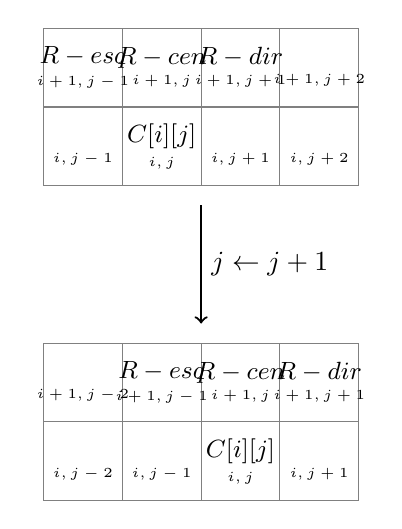
\begin{tikzpicture}
    \draw[step=\passo*2cm,color=gray] (-4*\passo,0*\passo) grid (4*\passo,4*\passo);
    \node at (-3*\passo,+3*\passo) {\cell[$\id{R-esq}$]{i+1,j-1}};
    \node at (-1*\passo,+3*\passo) {\cell[$\id{R-cen}$]{i+1,j}};
    \node at (+1*\passo,+3*\passo) {\cell[$\id{R-dir}$]{i+1,j+1}};
    \node at (+3*\passo,+3*\passo) {\cell{i+1,j+2}};
    \node at (-3*\passo,+1*\passo) {\cell{i,j-1}};
    \node at (-1*\passo,+1*\passo) {\cell[$C\chave{i}\chave{j}$]{i,j}};
    \node at (+1*\passo,+1*\passo) {\cell{i,j+1}};
    \node at (+3*\passo,+1*\passo) {\cell{i,j+2}};

    \draw [thick,->] (0*\passo, 0 *\passo - 0.5*\passo) -- (0*\passo, -4*\passo + 0.5*\passo) node[midway, right] {$j \gets j + 1$};

    \draw[step=\passo*2cm,color=gray] (-4*\passo,-8*\passo) grid (4*\passo,-4*\passo);
    \node at (-3*\passo,-5*\passo) {\cell{i+1,j-2}};
    \node at (-1*\passo,-5*\passo) {\cell[$\id{R-esq}$]{i+1,j-1}};
    \node at (+1*\passo,-5*\passo) {\cell[$\id{R-cen}$]{i+1,j}};
    \node at (+3*\passo,-5*\passo) {\cell[$\id{R-dir}$]{i+1,j+1}};
    \node at (-3*\passo,-7*\passo) {\cell{i,j-2}};
    \node at (-1*\passo,-7*\passo) {\cell{i,j-1}};
    \node at (+1*\passo,-7*\passo) {\cell[$C\chave{i}\chave{j}$]{i,j}};
    \node at (+3*\passo,-7*\passo) {\cell{i,j+1}};
\end{tikzpicture}